\documentclass[conference]{IEEEtran}
\IEEEoverridecommandlockouts
\usepackage{amsmath,amssymb}
\usepackage{graphicx}
\usepackage{booktabs}
\usepackage{cite}
\usepackage{microtype}
\usepackage{url}
\graphicspath{{figures/}}
\newcounter{algorithm}
\newcommand{\algorithmname}{Algorithm}
\newenvironment{IEEEalgorithm}[1]{%
  \refstepcounter{algorithm}%
  \begin{figure}[t]
  \hrule\vspace{2pt}
  \noindent\textbf{\algorithmname~\thealgorithm:} #1\par
  \vspace{2pt}\hrule\vspace{2pt}
  \normalsize
}{%
  \vspace{2pt}\hrule
  \end{figure}
}
\newcommand{\algline}[3]{%
  \noindent\makebox[1.35em][r]{#1}\hspace{0.35em}%
  \hspace*{#2em}#3\par
}

\title{A Tracking Method Based on Reinforcement Learning and Dynamic Cage Pose Reconstruction\thanks{Code available at \protect\url{https://github.com/JiarunSHI/PPO_caging_capture}.}}
\author{\IEEEauthorblockN{Jiarun Shi}
\IEEEauthorblockA{\textit{School of Information Science and Technology}\\
\textit{Beijing University of Chemical Technology}\\
Beijing, China\\
2023030094@buct.edu.cn}
\and
\IEEEauthorblockN{Xiaodong Feng\textsuperscript{*}}
\IEEEauthorblockA{\textit{School of Information Science and Technology}\\
\textit{Beijing University of Chemical Technology}\\
Beijing, China\\
2002500022@buct.edu.cn}
\thanks{\textsuperscript{*}Corresponding author: Xiaodong Feng.}
}

\begin{document}
\maketitle

\begin{abstract}
Continuous tracking of a moving object requires a manipulator to adjust its end-effector pose in time while maintaining a relative configuration that discourages target escape. Visual uncertainty, unavailable motion states, and limited manipulator response make conventional target-center following insufficient for simultaneously achieving tracking stability and agility. This paper presents a dynamic Cage pose reconstruction and staged-control framework for an eye-in-hand manipulator. In the offline stage, Cage-selection experience is acquired through dynamics simulation based on the actual gripper geometry. During online execution, the target motion trend is estimated from RGB-D observations, and the offline experience is used to reconstruct a motion-consistent Cage reference in real time. A model-based controller performs large-range pose adjustment, while a reinforcement-learning policy provides continuous local tracking, exploiting their complementary strengths in interpretability, stability, and responsive correction. MuJoCo experiments over trajectories with different spatial locations, speeds, and curvatures demonstrate the executability of the complete framework and its ability to provide stable and agile tracking in the presence of visual errors.
\end{abstract}

\begin{IEEEkeywords}
Dynamic caging, eye-in-hand vision, moving-target tracking, proximal policy optimization, visual motion estimation.
\end{IEEEkeywords}

\section{Introduction}

Continuous observation and manipulation of a moving object are fundamental to interception, in-motion handling, and close-range human--robot interaction. Unlike static reaching, the object continues to move while an image is acquired, processed, and converted into a robot command. A controller that reacts only to the latest measured center therefore accumulates delay-dependent tracking error. With an eye-in-hand camera, the same error can move the object outside both the observation field and the effective control range.

Moving-target visual servoing provides the closest background. Ito and Shibata compensated target motion in an image-based eye-in-hand controller for a planar hand--eye robot \cite{ito2009}. Shahriari \emph{et al.} treated target-induced feature motion as a disturbance, combining depth and motion observation with focus-of-expansion information \cite{shahriari2013}. These works demonstrate that motion estimation can reduce visual following delay, but their objectives are image-feature regulation rather than construction and tracking of a three-dimensional, motion-aware Cage reference.

In this work, a Cage denotes an open end-effector pose selected to be favorable for capture and unfavorable for target escape; it is not a sealed enclosure. Candidate quality is evaluated against the actual rear wall, open mouth, width, and height of the U-shaped gripper. The previously considered construction obtained by rotating the fingers by $\pm30^{\circ}$ to form a swept three-dimensional Cap is explicitly excluded. Offline dynamics simulation acquires Cage-selection experience, and online reconstruction reuses this experience without repeating the expensive candidate search.

The control problem spans two regimes. Differential Jacobian control produces an interpretable descent direction and rapidly handles a large pose discrepancy, whereas reinforcement learning can learn repeated local corrections under joint coupling and actuator dynamics. JAiLeR showed that task-space goals can be mapped to joint-space control through deep reinforcement learning \cite{kumar2021}; proximal policy optimization (PPO) supplies a conservative update for a continuous stochastic policy \cite{schulman2017ppo}. The proposed controller exploits these complementary properties: the Jacobian method performs coarse approach, and PPO supplies agile local tracking once the reconstructed Cage enters a prescribed neighborhood.

The main contributions are:
\begin{enumerate}
    \item an offline dynamics-based method that compares motion-consistent Cage candidates under identical disturbances and the true gripper geometry;
    \item a causal eye-in-hand pipeline combining RGB-D detection, five-frame state initialization, Kalman filtering, local spline fitting, and motion-plane estimation;
    \item a hybrid Jacobian--PPO controller with an explicit 18-dimensional state, dynamically scaled six-joint velocity action, independent Actor/Critic optimization, and staged exploration control; and
    \item an integrated MuJoCo implementation that retains perception errors and demonstrates the complete chain from offline experience acquisition to online reconstruction and hybrid tracking.
\end{enumerate}

\section{Related Work}

\subsection{Moving-Target Visual Servoing}

Moving targets introduce an external feature velocity that causes steady tracking lag if it is ignored. Ito and Shibata reduced this delay through target-motion compensation on a three-degree-of-freedom planar eye-in-hand robot \cite{ito2009}. Shahriari \emph{et al.} adapted a depth observer to a moving target, estimating image-plane motion through a disturbance observer and the orthogonal component through focus of expansion \cite{shahriari2013}. Dong and Zhu combined eye-in-hand visual servoing with adaptive extended Kalman estimation for autonomous capture \cite{dong2016}. These methods motivate the explicit separation of measurement filtering, motion estimation, reference generation, and robot control adopted here.

\subsection{Learned Joint-Space Control}

Inverse kinematics and Jacobian control are efficient and interpretable but require explicit treatment of singularities, joint limits, and velocity bounds. Learned joint-space control can represent nonlinear coupling directly. JAiLeR maps task-space goals and robot states to joint-space commands through model-free reinforcement learning and demonstrates sub-centimeter reaching in simulation and on hardware \cite{kumar2021}. EARL couples eye-in-hand pose tracking and dynamic grasping: four pose keypoints, their temporal change, and robot joint states are mapped by PPO to joint-velocity and gripper commands \cite{huang2023earl}. These systems learn position and orientation within one coupled pose representation. In contrast, the present policy is trained through masked-position, observed-position, and joint-pose passes. This ordering first establishes reaching, then exposes orientation observations, and finally optimizes coupled six-dimensional correction. The implementation further uses independent Actor and Critic optimizers, per-stage exploration scheduling, error-dependent physical action scaling, and online Jacobian--PPO mode switching.

\subsection{Dynamics-Based Cage Evaluation}

Geometric caging describes configurations that restrict object escape, while dynamic-caging analysis additionally studies robustness under motion and disturbances \cite{dong2024caging}. The present objective is narrower than constructing a globally closed cage: it ranks a finite set of open U-gripper poses for one local target-motion state. Repeated forward dynamics and identical disturbance tapes provide a controlled comparison, after which the offline result is compressed into a low-cost online prior.

\section{Problem Formulation and Architecture}

\subsection{Frames and Objective}

All frames are right-handed. Let $\{B\}$, $\{T\}$, $\{K\}$, and $\{G\}$ denote the robot Base, TCP, camera, and physical gripper Cage frames. The camera and gripper are rigidly attached to the terminal link, so \({}^{T}\mathbf T_K\) and \({}^{T}\mathbf T_G\) are fixed calibrations. The desired dynamic Cage pose \({}^{B}\mathbf T^{*}_{C,k}\), in contrast, changes with the observed motion.

The RGB-D detector returns the center of a spherical target proxy. In homogeneous coordinates,
\begin{equation}
{}^{B}\bar{\mathbf p}_{o,k}
= {}^{B}\mathbf T_{K,k}\,{}^{K}\bar{\mathbf p}_{o,k},
\qquad
{}^{B}\mathbf T_{K,k}
= {}^{B}\mathbf T_{T,k}\,{}^{T}\mathbf T_K .
\label{eq:camera_to_base}
\end{equation}
The physical MuJoCo object has mass, radius, contact, and rigid-body dynamics; only its center is required for online Cage reconstruction. The desired TCP pose is obtained through the fixed gripper extrinsic:
\begin{equation}
{}^{B}\mathbf T^{*}_{T,k}
= {}^{B}\mathbf T^{*}_{C,k}
\left({}^{T}\mathbf T_G\right)^{-1}.
\label{eq:cage_to_tcp}
\end{equation}
The robot tracks this pose subject to joint, rate, collision, workspace, and visibility constraints.

\subsection{Multi-Rate State Machine}

The RGB-D clock is 10~Hz, joint commands are updated at 100~Hz, and MuJoCo integrates at 500~Hz. Target motion is independent of inference. During the first five valid images, the robot holds an observation pose and collects raw visual centers. Starting at frame six, the system reconstructs the Cage and uses a bounded Jacobian controller. PPO is latched when the position and shortest-rotation errors fall below 15~mm and $45^{\circ}$, respectively. One or two missing images invoke state prediction; three consecutive misses terminate the simulated task. Table~\ref{tab:system_contract} summarizes the execution contract.

\begin{table}[t]
\caption{Core System Contract}
\label{tab:system_contract}
\centering
\begin{tabular}{lr}
\toprule
Quantity & Value \\
\midrule
RGB-D update & 100 ms (10 Hz) \\
Joint-control update & 10 ms (100 Hz) \\
MuJoCo integration step & 2 ms \\
Estimator state & 9 dimensions \\
PPO state/action & 18 / 6 dimensions \\
PPO entry neighborhood & 15 mm, $45^{\circ}$ \\
Visual failure & 3 consecutive misses \\
\bottomrule
\end{tabular}
\end{table}

\section{Visual Motion and Cage Reconstruction}

\subsection{RGB-D Measurement and State Initialization}

The simulation camera renders $320\times240$ color and depth images. A red-color mask isolates the spherical object; valid foreground pixels are back-projected, and their median three-dimensional point is offset by the known 18-mm radius along the viewing direction. Center estimation is therefore an RGB-D measurement process, not direct access to the MuJoCo state.

The first valid image defines the beginning of an observation sequence, but a velocity is neither measured nor assumed at that instant. At the 10-Hz visual rate, the five centers \(P_1,\ldots,P_5\) span four sampling intervals, i.e., 0.4~s. For the configured 0.11--0.18~m/s motion range, this corresponds to approximately 44--72~mm of traveled arc length. The interval is therefore long enough to expose a measurable motion trend while remaining local relative to the complete trajectory. The nine-dimensional motion state is
\begin{equation}
\mathbf x_k =
\begin{bmatrix}
\mathbf p_k^{\mathsf T}&
\mathbf v_k^{\mathsf T}&
\mathbf a_k^{\mathsf T}
\end{bmatrix}^{\mathsf T}.
\label{eq:motion_state}
\end{equation}
The five valid centers are fitted jointly by a local quadratic model whose time origin is the newest measurement. The fit therefore initializes position, velocity, and acceleration at \(P_5\), rather than attempting to assign a reliable velocity to \(P_1\). During bootstrap, the first-frame provisional velocity may be zero and intermediate finite-difference velocities are diagnostic only; no Cage command depends on them. Fit residuals initialize the covariance, with standard-deviation floors of 3~mm, 0.03~m/s, and 0.20~m/s$^2$. This history-based initialization avoids imposing zero target velocity on the formal filter state.

From frame six, a constant-acceleration Kalman model with white-jerk process noise performs prediction and position correction \cite{kalman1960}. The innovation is accepted only when
\begin{equation}
d_k^2=\mathbf y_k^{\mathsf T}\mathbf S_k^{-1}\mathbf y_k
\leq 14.16.
\label{eq:innovation_gate}
\end{equation}
A missed or rejected measurement invokes prediction only and increases uncertainty; it does not erase the accumulated state. The configured observation variance is $9\times10^{-6}$~m$^2$.

\subsection{Causal Spline and Local Motion Plane}

A cubic B-spline is fitted over a finite causal window. The three coordinates share timestamps, knots, basis functions, and recency weights. The implemented fit is
\begin{equation}
\mathbf C^{*}=\arg\min_{\mathbf C}
\sum_i w_i
\left\|\mathbf b(t_i)^{\mathsf T}\mathbf C-\hat{\mathbf p}_i\right\|_2^2
+\lambda\left\|\mathbf D_2\mathbf C\right\|_F^2 ,
\label{eq:spline}
\end{equation}
where $\mathbf D_2$ penalizes second differences of the control coefficients. Kalman state variables provide online position, velocity, and acceleration; the spline supplies causal curve continuation, tangent fallback, and curvature
\begin{equation}
\kappa(t)=
\frac{\left\|\dot{\mathbf s}(t)\times\ddot{\mathbf s}(t)\right\|_2}
{\left\|\dot{\mathbf s}(t)\right\|_2^3}.
\label{eq:curvature}
\end{equation}

The centered covariance of recent curve samples has eigenvalues
$\lambda_1\leq\lambda_2\leq\lambda_3$. When $\lambda_2/\lambda_3$ indicates sufficient two-dimensional spread, the eigenvector of $\lambda_1$ defines the PCA plane normal \cite{jolliffe2002}. For sufficiently curved motion, the differential normal $\dot{\mathbf s}\times\ddot{\mathbf s}$ is also available. Near a line, the previous normal or a Base-frame reference is reused. Sign consistency and rotation bounds prevent eigenvector flips.

\subsection{Speed-Dependent Minor Arc}

The target center is the center of a candidate circle in the local motion plane. Its unfiltered speed-dependent radius is
\begin{equation}
\tilde r_k=0.10+
0.08\,\operatorname{clip}\!\left(
\frac{\|\mathbf v_k\|-0.05}{0.45-0.05},0,1
\right)\ \mathrm{m}.
\label{eq:speed_radius}
\end{equation}
At 10~Hz, $r_k=0.49r_{k-1}+0.51\tilde r_k$, followed by a physical rate limit of 0.18~m/s. The tangent--circle intersection defines the arc start; the first intersection of the causally continued curve and circle defines the end. For normalized coordinate $\alpha\in[0,1]$,
\begin{align}
\theta(\alpha)&=\theta_s+\alpha(\theta_e-\theta_s),\nonumber\\
\mathbf p_C(\alpha)&=\mathbf p_k+r_k
\left[\cos\theta(\alpha)\mathbf u_k+
\sin\theta(\alpha)\mathbf v_k\right].
\label{eq:arc}
\end{align}
The Cage $x$-axis points toward the object, its $z$-axis is the stabilized positive plane normal, and its $y$-axis completes a right-handed frame. Hence the Cage $x$--$y$ plane is parallel to the local motion plane.

\section{Offline Dynamics-Based Cage Experience}

\subsection{Candidates and EST Expansion}

For offline experience generation, the first five trajectory points are retained as causal geometric history but do not produce Cage labels. The first valid label is generated at \(P_6\). Because \(P_1\) to \(P_6\) spans five 0.1-s intervals, the clean object has traveled approximately 55--90~mm before the first label under the configured speed range. Velocity, acceleration, tangent, and curvature at \(P_6\) are obtained from the smooth trajectory fit rather than from a separately specified first-frame velocity. Nine candidates then uniformly sample the exact minor arc. The clean generated trajectory supplies the privileged future segment needed to locate the arc endpoint; this is confined to offline label construction. Online reconstruction uses only causal spline continuation.

One candidate remains fixed during each EST trial, in contrast to dynamic-caging robustness analysis that perturbs motion under forward dynamics and energy margins \cite{dong2024caging}. The root contains current object position and linear velocity. Following the expansive-space-tree principle \cite{hsu1997}, EST selects parents preferentially from sparsely occupied cells of a position--linear-velocity--angular-velocity grid. A random force, torque, and duration are applied, and MuJoCo performs forward integration. Seventy percent of force directions point into the current motion-arc sector, while 30\% preserve global three-dimensional exploration. Each candidate receives the same three disturbance tapes, 640 nodes per repeat, a 0.8-s horizon, and a 5-ms integration step.

Valid states are classified against the actual rear wall, open mouth, width, and height of the U-shaped gripper. Nonfinite states, local-bound violations, and penetration beyond 6~mm are not expanded.

Algorithm~\ref{alg:est} summarizes this fixed-candidate expansion.

\begin{IEEEalgorithm}{Offline EST Evaluation of Fixed Cage Candidates}
\label{alg:est}
\noindent\textbf{Input:} fitted geometric target state $\mathbf{x}_{k}$; candidate poses $\mathcal{C}$; gripper geometry $\mathcal{G}$; shared disturbance tape $\mathcal{D}$\par
\noindent\textbf{Output:} selected candidate $j^{*}$ and fixed online arc prior $\alpha^{*}$\par
\noindent\textbf{Data:} $M=3$ repeats; $N_{\max}=640$ nodes; $T_{\max}=0.8$~s; step $5$~ms\par
\algline{1}{0}{\textbf{for} each candidate $j\in\mathcal{C}$ \textbf{do}}
\algline{2}{1}{\textbf{for} $m=1,\ldots,M$ \textbf{do}}
\algline{3}{2}{$\mathcal{T}\leftarrow\{\operatorname{root}(\mathbf{x}_k)\}$; initialize density grid}
\algline{4}{2}{\textbf{while} $|\mathcal{T}|<N_{\max}$ and horizon $<T_{\max}$ \textbf{do}}
\algline{5}{3}{$\mathbf{x}_{\mathrm{parent}}\leftarrow\operatorname{sampleLowDensity}(\mathcal{T})$}
\algline{6}{3}{$(\mathbf{f},\boldsymbol{\tau},\Delta t)\leftarrow\mathcal{D}[m,|\mathcal{T}|]$}
\algline{7}{3}{$\mathbf{x}_{\mathrm{new}}\leftarrow\operatorname{propagate}(\mathbf{x}_{\mathrm{parent}},\mathbf{f},\boldsymbol{\tau},\Delta t)$}
\algline{8}{3}{\textbf{if} finite$(\mathbf{x}_{\mathrm{new}})$ and legal$(\mathbf{x}_{\mathrm{new}})$ \textbf{then}}
\algline{9}{4}{add $\mathbf{x}_{\mathrm{new}}$ to $\mathcal{T}$; update density}
\algline{10}{3}{\textbf{end if}}
\algline{11}{2}{\textbf{end while}}
\algline{12}{2}{$\rho_{j,m}\leftarrow\operatorname{countInside}(\mathcal{T},\mathcal{G},\mathcal{C}_{j})/|\mathcal{T}|$}
\algline{13}{1}{\textbf{end for}}
\algline{14}{1}{$\bar{\rho}_{j}\leftarrow\operatorname{mean}(\rho_{j,1:M})$; $\sigma_j\leftarrow\operatorname{std}(\rho_{j,1:M})$}
\algline{15}{0}{\textbf{end for}}
\algline{16}{0}{$j^{*}\leftarrow\arg\max_{j\in\mathcal F}\bar{\rho}_{j}$; use candidate index only for an exact tie}
\algline{17}{0}{$\alpha^{*}\leftarrow\operatorname{midpoint}\bigl(\operatorname{median}(\alpha),\,0.5\bigr)$}
\algline{18}{0}{\textbf{return} $j^{*}$ and $\alpha^{*}$}
\end{IEEEalgorithm}

For candidate $j$ and repeat $m$,
\begin{equation}
\rho_{j,m}=\frac{N^{\mathrm{in}}_{j,m}}{N_{j,m}},
\quad
\bar\rho_j=\frac{1}{3}\sum_{m=1}^{3}\rho_{j,m},
\quad
\sigma_j=\operatorname{Std}(\rho_{j,1:3}).
\label{eq:est_score}
\end{equation}
The final label is
\begin{equation}
j^{*}=\arg\max_{j\in\mathcal F}\bar\rho_j ,
\label{eq:est_selection}
\end{equation}
where $\mathcal F$ is the feasible set and the winner must exceed the nonzero-retention threshold. IK margin, joint change, temporal continuity, pose smoothness, and arc midpoint are not secondary ranking terms; the candidate index only resolves an exact tie.

\subsection{Compact Online Prior}

The archive contains 55,121 valid labels from 2,919 trajectories. The winning $\alpha$ has mean 0.402 and median 0.375. An all-candidate audit of 10,000 labels shows that fixed $\alpha=0.5$ has the largest mean occupancy. Absolute correlations of the winner with speed, acceleration, curvature, and radius are below 0.02. Figure~\ref{fig:est_statistics} therefore supports a fixed prior more strongly than a learned arc regressor for the present gripper and disturbance distribution. The online reconstruction uses $\alpha=0.4375$, halfway between the empirical median and the best fixed audit candidate.

\begin{figure*}[t]
\centering
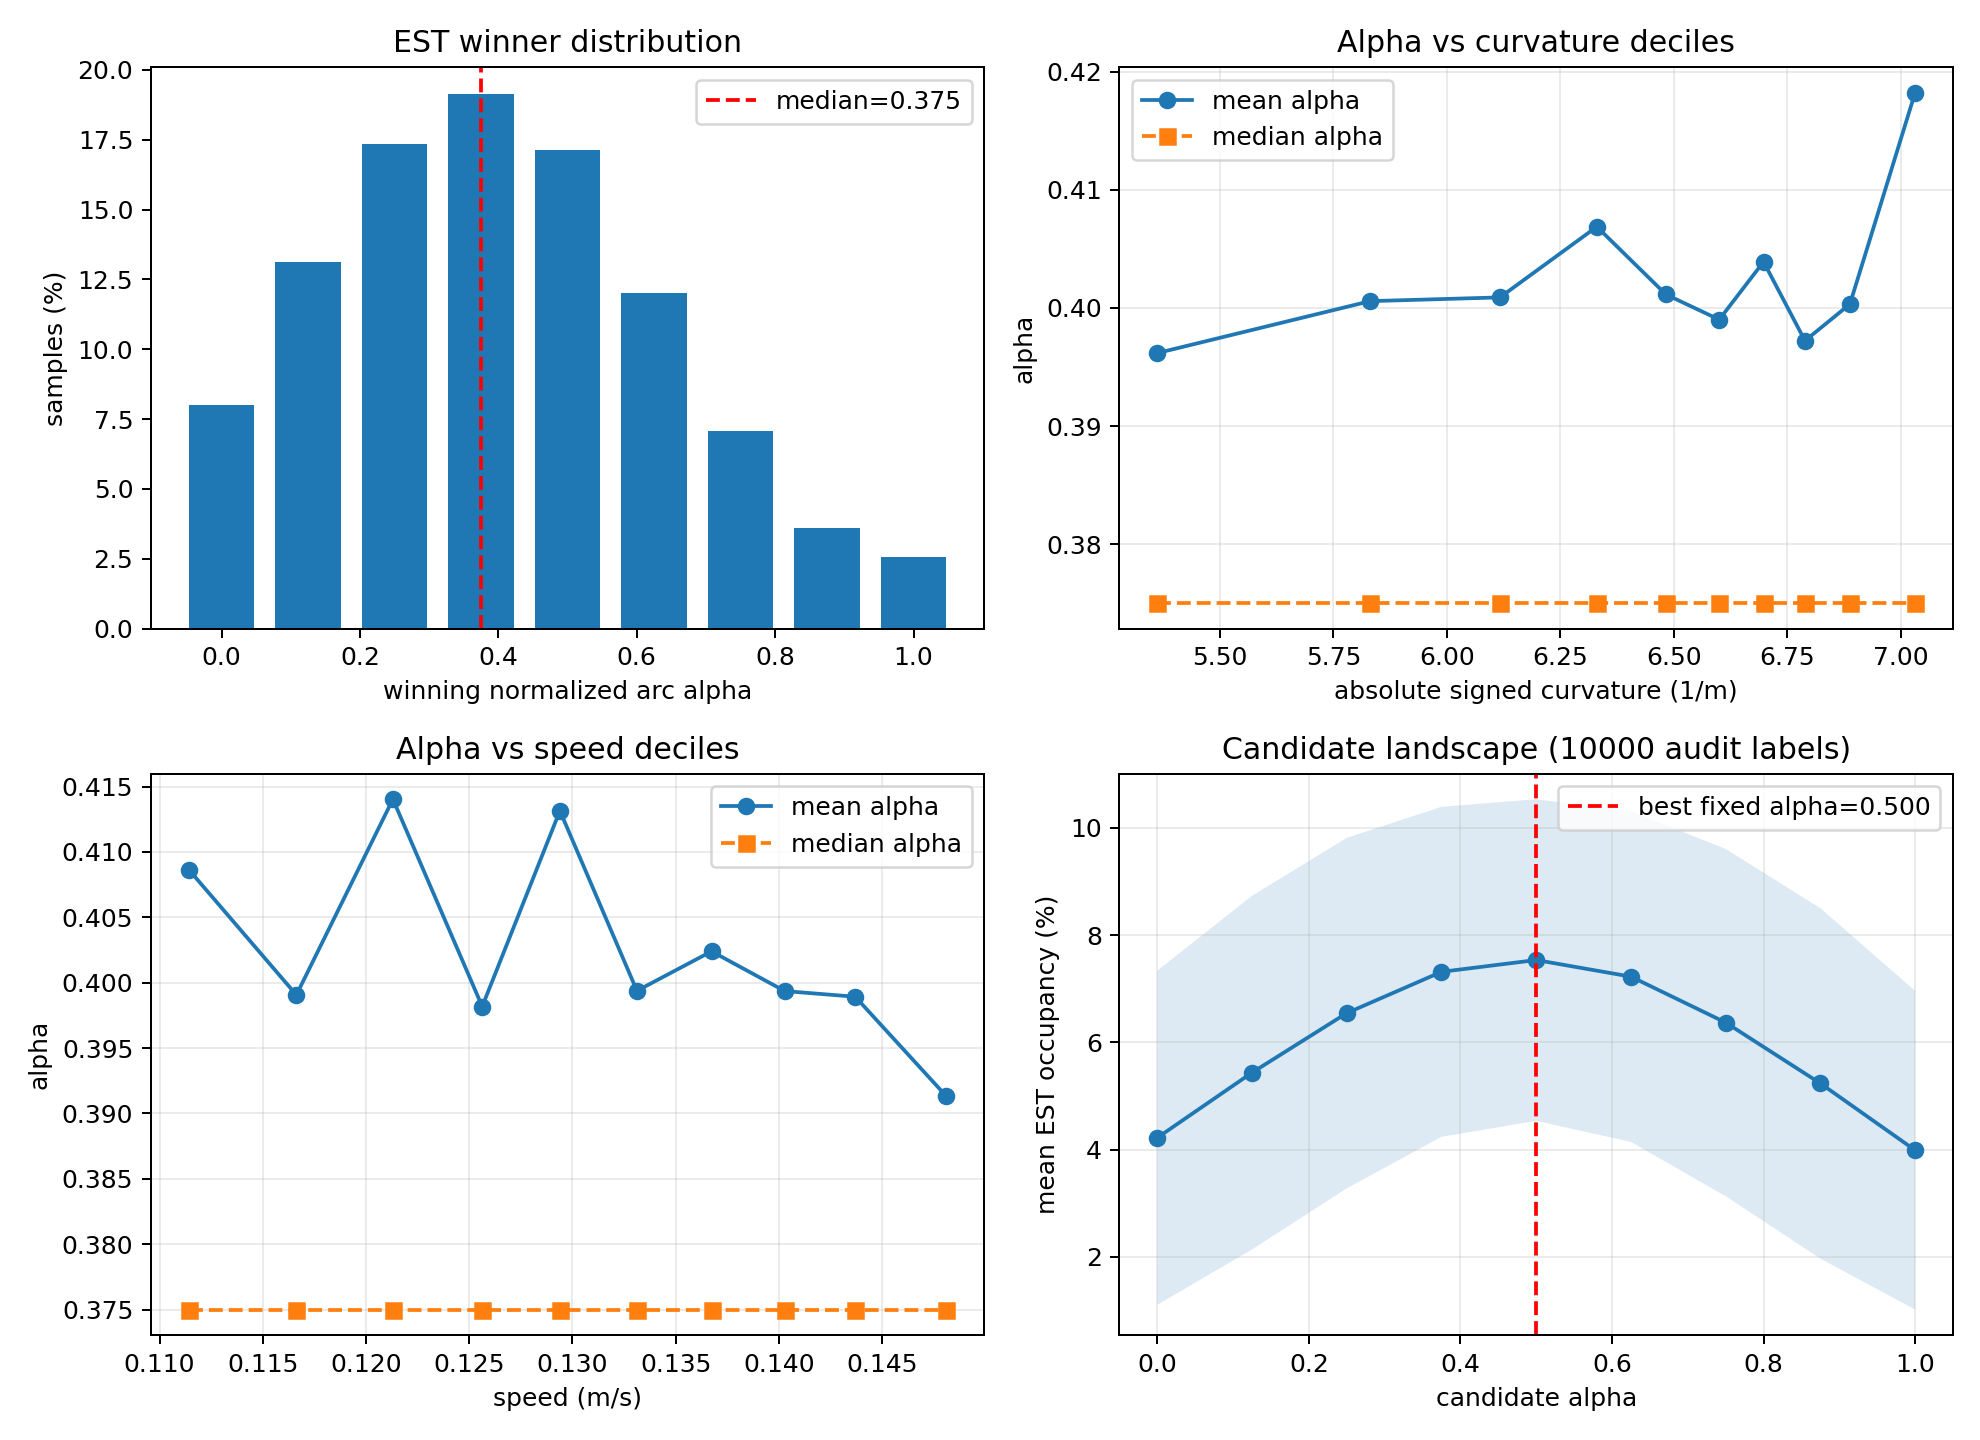
\includegraphics[width=0.88\textwidth]{state_arc_prior_relationships.png}
\caption{Offline EST statistics. Winners cluster near the middle of the minor arc, whereas dependence on speed and curvature is weak; the fixed prior is therefore better supported than a learned arc regressor.}
\label{fig:est_statistics}
\end{figure*}

\section{Hybrid Control and Policy Training}

\subsection{Bounded Jacobian Approach}

Let $\mathbf e_p$ be the Base-frame TCP position error and $\mathbf e_R$ the shortest rotation-vector error. The desired Cartesian twist is
\begin{equation}
\boldsymbol\xi^{*}=\boldsymbol\xi_{\mathrm{ff}}+
\begin{bmatrix}k_p\mathbf e_p&k_R\mathbf e_R\end{bmatrix}^{\mathsf T}.
\label{eq:twist}
\end{equation}
The approach controller solves a bounded damped least-squares problem \cite{wampler1986}:
\begin{equation}
\dot{\mathbf q}^{*}=
\arg\min_{\dot{\mathbf q}}
\|\mathbf W(\mathbf J\dot{\mathbf q}-\boldsymbol\xi^{*})\|_2^2
+\lambda_J\|\dot{\mathbf q}\|_2^2 ,
\;
\dot{\mathbf q}_{\min}\leq\dot{\mathbf q}\leq\dot{\mathbf q}_{\max}.
\label{eq:jacobian}
\end{equation}
The bounds include speed, acceleration, and remaining joint-position margins. This phase provides predictable large-error convergence without requiring PPO to discover long-range inverse kinematics.

\subsection{PPO State, Network, and Action}

The policy state is
\begin{equation}
\mathbf s_t=
\begin{bmatrix}
\mathbf e_{p,t}^{\mathsf T}&
\mathbf e_{R,t}^{\mathsf T}&
\mathbf q_t^{\mathsf T}&
\dot{\mathbf q}_t^{\mathsf T}
\end{bmatrix}^{\mathsf T}\in\mathbb R^{18}.
\label{eq:ppo_state}
\end{equation}
Running means and variances normalize the state. Actor and Critic have independent $18\!\rightarrow\!128\!\rightarrow\!128$ multilayer perceptrons with $\tanh$ hidden activations. The Actor outputs six means and maintains six trainable state-independent log standard deviations; the Critic outputs one state value. Figure~\ref{fig:ppo_training} summarizes the training loop and curriculum update.

\begin{figure}[t]
\centering
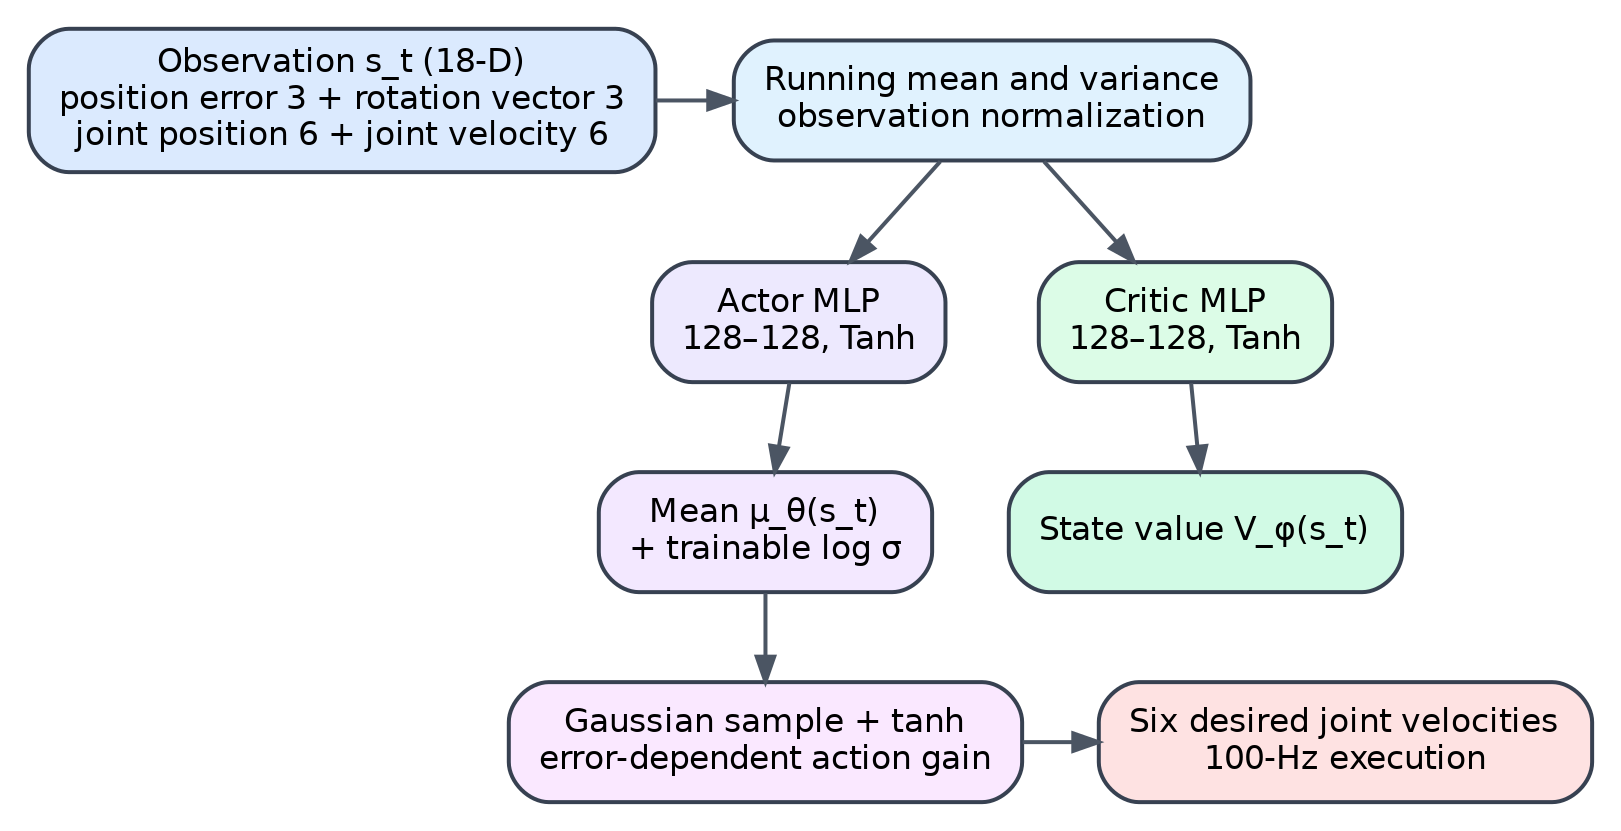
\includegraphics[width=\columnwidth]{ppo_architecture_en.png}
\caption{Independent Actor--Critic architecture. The Actor produces a squashed six-joint velocity command, while the Critic estimates the state value from the same normalized observation.}
\label{fig:ppo_training}
\end{figure}

The latent action is sampled as $\mathbf u_t\sim\mathcal N(\boldsymbol\mu_\theta(\bar{\mathbf s}_t),\operatorname{diag}(\boldsymbol\sigma_\theta^2))$ and squashed to $\mathbf a_t=\tanh(\mathbf u_t)$. Here, $\bar{\mathbf s}_t$ is the normalized state, $\boldsymbol\mu_\theta$ is the Actor mean, and $\boldsymbol\sigma_\theta$ is obtained from the trainable log standard deviation. Its change-of-variables log density is
\begin{equation}
\log\pi_\theta(\mathbf a_t|\mathbf s_t)=\log\mathcal N(\operatorname{atanh}\mathbf a_t;
\boldsymbol\mu_\theta,\boldsymbol\sigma_\theta)
-\sum_i\log(1-a_{t,i}^2+\varepsilon).
\label{eq:action}
\end{equation}
The final sum is the Jacobian correction for the $\tanh$ mapping, and $\varepsilon$ is a small numerical constant. It converts the Gaussian density of the latent action into the density of the actually executed bounded action.

The policy output is a normalized joint velocity, not a one-step target displacement. At every 10-ms control step, the larger of the position and orientation errors after normalization by the current task tolerances selects one common physical gain. The gain is linearly interpolated from 0.10 near the target to 1.00 at six tolerance units and is capped by the current curriculum stage; position-only stages omit the orientation ratio. The six bounded actions are then multiplied elementwise by the UR5e joint-velocity limits and this common gain. Consequently, the same normalized policy command produces gentle motion near the goal and faster motion at large error without changing the policy distribution used by PPO.

\subsection{PPO, Critic, and Exploration Entropy}

After every rollout, generalized advantages (GAE) \cite{schulman2015gae} are computed once from the frozen pre-update value network:
\begin{align}
\delta_t&=r_t+\gamma(1-b_t)V_{\mathrm{old}}(s_{t+1})
-V_{\mathrm{old}}(s_t),\nonumber\\
\hat A_t&=\delta_t+\gamma\lambda(1-d_t)\hat A_{t+1}.
\label{eq:gae}
\end{align}
Here, $\gamma$ is the discount factor, $\lambda$ is the GAE trace parameter, $b_t=1$ only for a true physical or task terminal, and $d_t=1$ at every sequence boundary. Success, collision, workspace violation, or a nonfinite state therefore removes the bootstrap value. A task time limit or rollout truncation stops advantage recursion so that samples from different tasks or logical slots never mix, but retains $V_{\mathrm{old}}(s_{t+1})$. The resulting advantages and Critic regression targets are fixed through all minibatch epochs of that update.

With probability ratio $\varrho_t(\theta)=\pi_\theta(a_t|s_t)/\pi_{\mathrm{old}}(a_t|s_t)$, the Actor maximizes
\begin{equation}
\begin{gathered}
J_\pi(\theta)=\mathbb E_t\Bigl[
\min\Bigl(\varrho_t\hat A_t^n,\operatorname{clip}(\varrho_t,1-\epsilon,1+\epsilon)\hat A_t^n\Bigr)\\
+\beta\mathcal H(\pi_\theta)\Bigr],
\end{gathered}
\label{eq:ppo}
\end{equation}
where $\hat A_t^n$ is normalized and
$\mathcal H=-\mathbb E_{\pi_\theta}[\log\pi_\theta]$ is evaluated for the squashed policy. The Critic independently minimizes
\begin{equation}
L_V(\phi)=\frac{1}{2}\mathbb E_t
\left[(V_\phi(s_t)-\hat V_t)^2\right].
\label{eq:critic}
\end{equation}
Here, $\hat V_t$ denotes the frozen GAE-derived regression target for the current update.
Separate Adam optimizers use learning rates $2\times10^{-5}$ and $10^{-4}$. Each update permits eight Actor epochs and twelve Critic epochs with 512-sample minibatches. PPO uses $\epsilon=0.2$. Approximate KL $\widehat D_{\mathrm{KL}}=\mathbb E_t[(\varrho_t-1)-\log \varrho_t]$ above 0.03 stops only Actor epochs; Critic regression continues. Clipping is therefore a local sample-wise restriction, while KL stopping limits the aggregate policy change.

Within each individual curriculum stage $s$ (for example, J04 rather than the complete joint-pose pass), the entropy coefficient follows
\begin{equation}
\begin{gathered}
\beta_s(n)=m_s(n)\!\left[
\beta_s^{0}+
\min\!\left(\frac{n}{N_s},1\right)
(\beta_s^{1}-\beta_s^{0})
\right],\\
\beta_s^{1}=\frac{1}{2}\beta_s^{0}.
\end{gathered}
\label{eq:entropy}
\end{equation}
Start values increase with task range: 0.0008--0.0018 in position passes and 0.0010--0.0030 in pose stages. The schedule encourages diverse actions early in each stage and precision later. After 20 updates with less than 2\% improvement, a pre-update Critic explained variance of at least 0.30 permits a 20-update entropy pulse $m_s=1.5$, at most three times per stage. A performance regression larger than 1\% never triggers more exploration because it is treated as possible policy--value instability rather than evidence of insufficient action diversity; increasing entropy in that case would amplify the degradation. The trainable log standard deviations are optimized by \eqref{eq:ppo}; the plateau detector does not permanently overwrite them.

\subsection{Overall Reward}

The reward assigned to the transition $(s_t,a_t,s_{t+1})$ is
\begin{equation}
\begin{gathered}
r_t=0.1\left(w_pQ_p+w_RQ_R-1\right)
+2w_pP_p+4w_RP_R\\
-0.001C_a+R_{\mathrm{term}}.
\end{gathered}
\label{eq:reward}
\end{equation}
The masked- and observed-position passes use $(w_p,w_R)=(1,0)$, so only position quality and position progress guide the task. The joint-pose pass activates both components and dynamically redistributes their weights toward the less accurate component. In \eqref{eq:reward}, $Q_p$ and $Q_R$ are bounded pose qualities, $P_p$ and $P_R$ are signed one-step progress terms, $C_a$ is normalized desired joint-acceleration cost, and $R_{\mathrm{term}}$ contains success and failure events.

For $e_p=\|\mathbf e_p\|_2$, position quality combines a millimeter-sensitive term and a long-tail term:
\begin{equation}
\begin{aligned}
Q_{p,f}&=\exp\!\left[-\ln 2\,(e_p/\delta_p)^2\right],\\
Q_{p,c}&=\frac{1}{1+(e_p/e_{p,\max})^2},\\
Q_p&=0.7Q_{p,f}+0.3Q_{p,c}.
\end{aligned}
\label{eq:position_quality}
\end{equation}
Here, $\delta_p$ is the current per-task position tolerance and $e_{p,\max}$ is the stage's maximum initial position error. The fine term equals 0.5 at $e_p=\delta_p$ and distinguishes nearby millimeter errors. The inverse-quadratic term remains informative at longer range, where the narrow exponential alone would make different poor states nearly indistinguishable. Their 0.7/0.3 weighting therefore combines precision near success with a usable descent signal over the complete curriculum range.

Orientation uses three 5-cm virtual markers anchored at one common origin:
\begin{equation}
\begin{aligned}
E_R&=\frac{1}{3}\sum_{i=1}^{3}
\|\ell\mathbf R\mathbf e_i-\ell\mathbf R^*\mathbf e_i\|_2^2,\\
Q_R&=\frac{1}{1+40000E_R},\qquad \ell=0.05\ \mathrm m.
\end{aligned}
\label{eq:orientation_quality}
\end{equation}
where $\mathbf R$ and $\mathbf R^*$ are the current and desired TCP rotations, $\mathbf e_i$ are the Cartesian basis vectors, and $\ell$ is the virtual-marker radius. The common origin prevents translation from being counted twice, and the inverse-quadratic quality retains variation after large wrist errors.

In pose stages, let $u_p=e_p/\delta_p$ and
$u_R=e_R^{\mathrm{deg}}/\delta_R$. Before either component succeeds,
$w_R=\operatorname{clip}(u_R/(u_p+u_R),0.25,0.75)$ and $w_p=1-w_R$.
If exactly one component succeeds, it retains weight 0.25 and the unfinished component receives 0.75; both receive 0.5 after joint success. Position stages use $(w_p,w_R)=(1,0)$.

The progress terms compare the error before and after the applied action: position improvement is divided by 5~mm and orientation improvement by $10^{\circ}$, then each term is clipped to $[-1,1]$. Once one component satisfies its tolerance, its positive progress is removed but any regression remains negative. This prevents repeated reward for oscillating inside a solved coordinate while still penalizing loss of accuracy. The quality term remains active with a smaller weight, so maintaining an already solved component still matters. Success adds $+10$. Collision, workspace violation, or a nonfinite state adds $-10$ plus the discounted remaining baseline cost; this compensation prevents an agent from terminating early merely to avoid future per-step penalties. A timeout is a sequence boundary rather than a physical failure and retains value bootstrap.

\subsection{Curriculum}

Fifty logical slots maintain independent UR5e states and randomized targets. Each completed task contributes one success or failure event, so a quickly solved task cannot be repeatedly counted as several successes. Table~\ref{tab:curriculum} summarizes 30 stages. In every pass, the maximum initial position error increases through 20, 32, 45, 60, 75, 90, 105, 120, 135, and 150~mm. The joint-pose pass simultaneously increases the maximum initial rotation through $5$, $8$, $11$, $15$, $19$, $24$, $29$, $35$, $40$, and $45^{\circ}$. The masked pass first learns position control with the three rotation-error inputs set to zero. The observed pass exposes those inputs while retaining a position-only objective. At each pass transition, Actor weights are retained, both Adam histories are cleared, and a newly initialized Critic is aligned to rollouts from the new observation/reward distribution. The joint pass then optimizes coupled position and orientation correction.

Task success requires the stage-specific error thresholds in Table~\ref{tab:curriculum} and terminal TCP linear speed below 0.08~m/s; joint-pose tasks additionally require angular speed below 0.30~rad/s. Thus the last-ten-update success rate used for promotion already includes final reach speed, rather than checking pose error alone. Promotion requires at least 75\% completed-task success and the corresponding last-ten mean error limits. Slot boundaries and unfinished rollout boundaries are passed to the two-mask GAE rule in \eqref{eq:gae}, preventing cross-task leakage while retaining bootstrap at time limits.

\begin{table*}[t]
\caption{Curriculum Ranges and Promotion Contract}
\label{tab:curriculum}
\centering
\footnotesize
\setlength{\tabcolsep}{3pt}
\begin{tabular}{@{}lccclp{5.3cm}@{}}
\toprule
Pass & Stages & Initial position & Initial rotation & Horizon & Success and promotion contract \\
\midrule
Masked position & M01--M10 & 6--20 to 6--150 mm & masked & 80--200 & Per-task position: 1.5--4.0 mm. Promote when last-10 success is at least 75\% and mean position is 2.3--8.0 mm. \\
Observed position & V01--V10 & 6--20 to 6--150 mm & observed & 80--200 & Same position-only contract; rotation enters the observation but not the success test. \\
Joint pose & J01--J10 & 6--20 to 6--150 mm & 0.5--5 to 0.5--45$^{\circ}$ & 100--250 & Per-task: 1.5--4.0 mm and 2.8--4.5$^{\circ}$. Promote at 75\% with means 2.3--8.0 mm and 3.4--6.5$^{\circ}$. \\
\bottomrule
\end{tabular}
\end{table*}

\subsection{Curriculum Training Results}

The completed run contains 34,745 updates and passes all 30 stages. Figure~\ref{fig:curriculum_results} reports equally weighted last-ten-update statistics and promotion boundaries. The best final-stage checkpoint occurs at update 34,547. Table~\ref{tab:best} reports its completed-task result: 92\% success, 2.95-mm mean terminal position error, 3.94$^{\circ}$ mean terminal rotation error, 1.97\% action saturation, and 0.997 post-update Critic explained variance. These values characterize randomized curriculum-reaching tasks; they are not presented as dynamic-trajectory generalization results.

\begin{figure}[t]
\centering
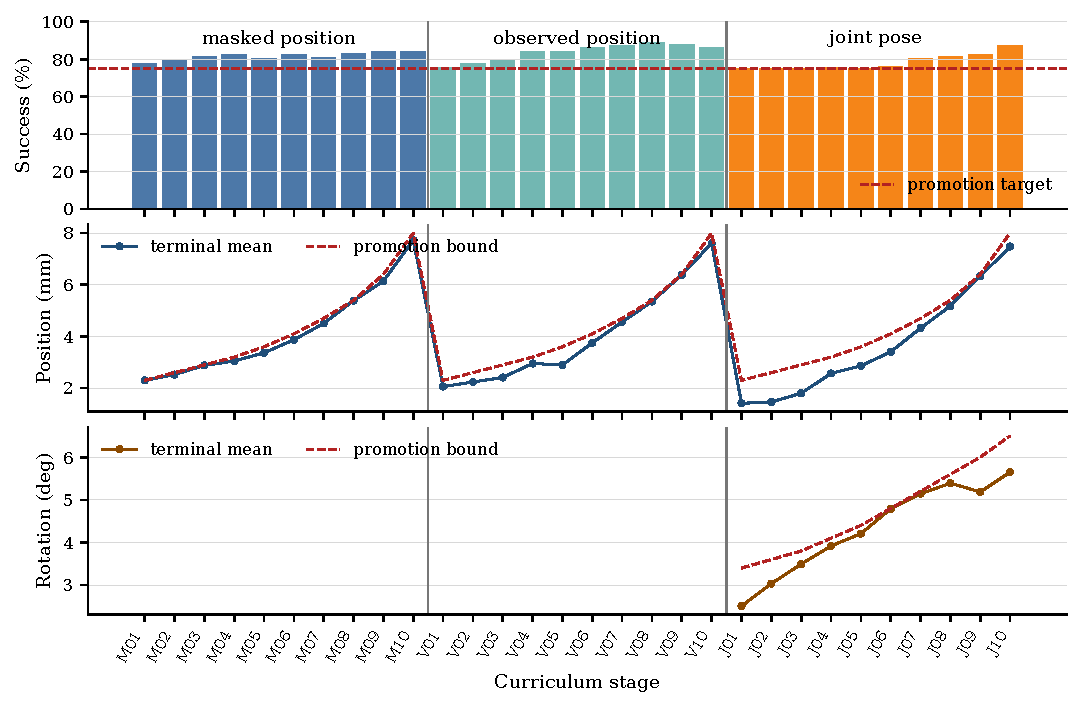
\includegraphics[width=\columnwidth]{curriculum_summary_ieee.pdf}
\caption{Per-stage curriculum summary over the last ten updates. Masked-position, observed-position, and joint-pose stages progressively expand the target range while retaining the 75\% promotion objective.}
\label{fig:curriculum_results}

\medskip

\refstepcounter{table}\label{tab:best}
{\scshape TABLE \thetable}\\
{\scshape Best Final-Stage Checkpoint}\\
\medskip
\begin{tabular}{lr}
\toprule
Metric & Result \\
\midrule
Completed-task success & 92\% \\
Position mean / P95 & 2.95 / 4.00 mm \\
Rotation mean / P95 & 3.94 / 4.83$^{\circ}$ \\
Action saturation & 1.97\% \\
Critic explained variance & 0.997 \\
\bottomrule
\end{tabular}
\end{figure}

\section{Experiments}

\subsection{Simulation and Perception Errors}

Experiments use the MuJoCo UR5e model \cite{todorov2012}, \texttt{attachment\_site} as TCP, a rigid U-shaped gripper, and an eye-in-hand camera. Dynamic trajectories last 5--7~s, have speed 0.11--0.18~m/s with 10\%--20\% smooth modulation, and are filtered for workspace and visibility. Their generated coordinates are hidden from online estimation.

The rendered measurements contain 2-mm depth noise, 1\% pixel-depth dropout, finite-resolution quantization, and 1\% whole-frame dropout. These errors change both position measurements and derived motion quantities, so Kalman filtering is not a cosmetic post-process: it estimates unobserved velocity and acceleration, propagates through short misses, and weights inconsistent centers through \eqref{eq:innovation_gate}. This paper does not claim a numerical advantage over a no-filter baseline, because that ablation remains to be conducted.

Three evidence levels are kept separate. The EST archive supports the arc prior. Curriculum rollouts characterize randomized Cage-reaching tasks and are not reported as dynamic-tracking generalization. A controlled ten-trajectory suite is used to demonstrate the integrated noisy RGB-D, online reconstruction, and hybrid-control pipeline. The experiment is an internal quantitative characterization of the proposed method rather than a comparative benchmark.

\subsection{Full Online Inference Process}

The complete causal flow is shown in Fig.~\ref{fig:inference_schedule}. RGB-D detection begins at the first trajectory sample. Frames 1--5 retain the observation pose and provide only measured centers for the quadratic state initialization. From frame six onward, prediction, innovation-gated correction, causal spline and plane fitting, Cage reconstruction, and control are executed. The bounded Jacobian controller is used outside the 15-mm/$45^{\circ}$ entry neighborhood; after both conditions are met, PPO is latched for 100-Hz local correction. The target motion and camera rendering continue independently in all phases.

\begin{figure*}[t]
\centering
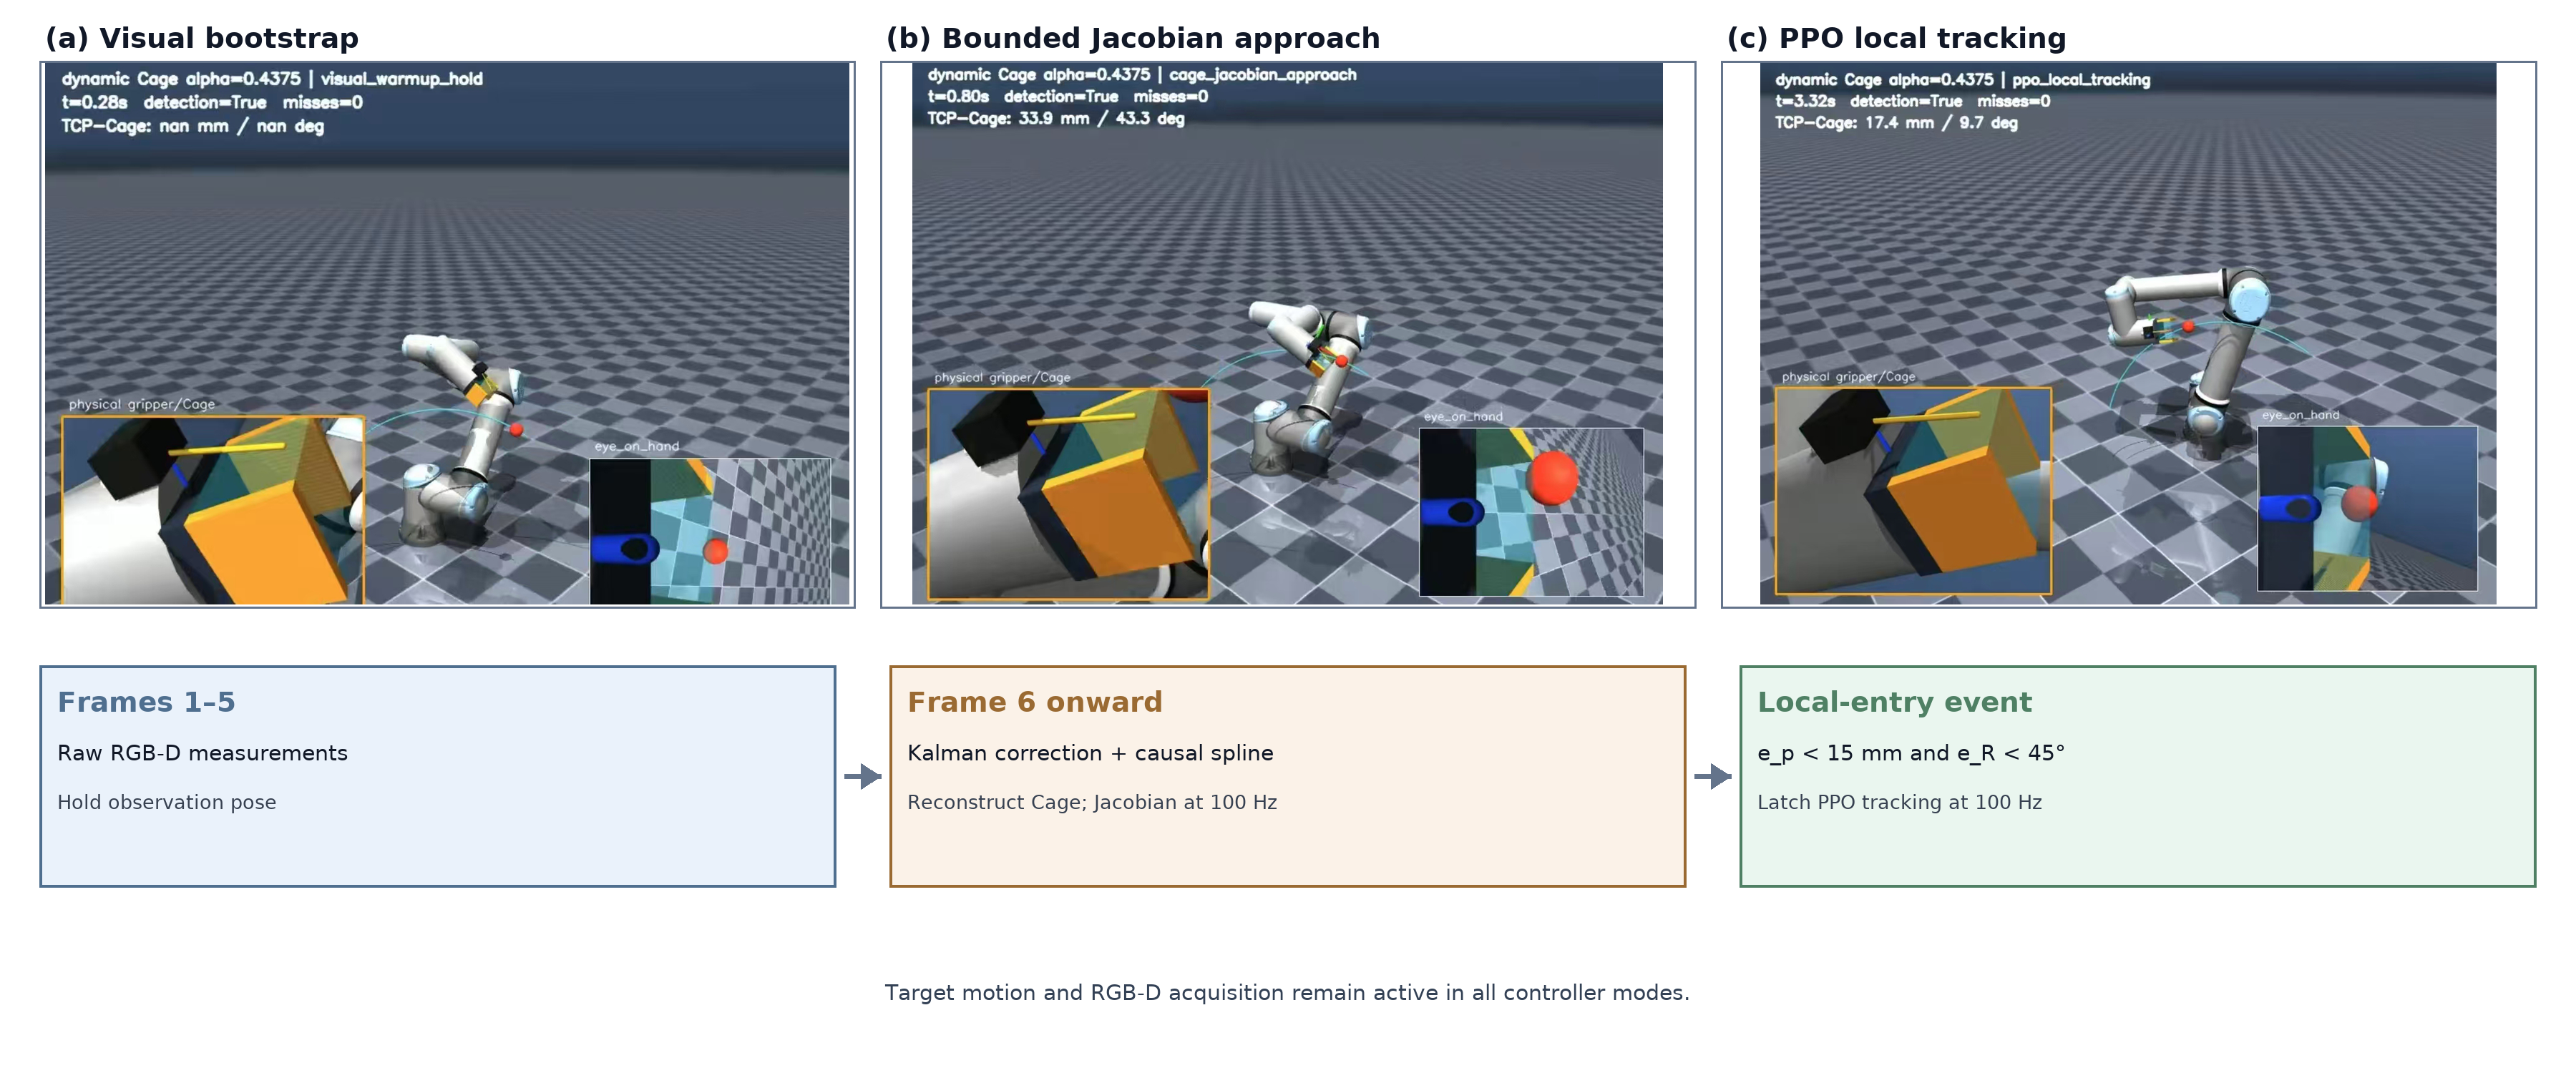
\includegraphics[width=0.96\textwidth]{inference_state_machine.png}
\caption{Causal online inference sequence. RGB-D measurements arrive every 100~ms; after the five-frame bootstrap, estimation, Cage reconstruction, and hybrid control operate without future samples.}
\label{fig:inference_schedule}
\end{figure*}

\subsection{Validation Trajectory Protocol}

The validation suite contains ten deterministic open trajectories selected with seeds 20261020--20261029, which are disjoint from offline EST and policy training. Rather than drawing ten nearly identical random curves, the generator assigns each seed a controlled spatial and motion profile. The profiles cover left, center, and right regions; low, middle, and elevated heights; low, medium, and high curvature; increasing and decreasing curvature trends; alternating turning directions; and three overlapping speed bands within 0.11--0.18~m/s. Table~\ref{tab:validation_profiles} summarizes this distribution. The paths are nonclosed, their speed varies smoothly, and their initial five-frame observation window must be visible. Workspace rejection additionally requires a minimum Base distance of 0.46~m, a minimum horizontal distance from the Base axis of 0.40~m, a maximum Base distance of 0.88~m, and a height between 0.24 and 0.68~m. These rules prevent trivial near-Base paths and unreachable far-field paths while retaining meaningful variation in position, direction, speed, and curvature.

\begin{table*}[t]
\caption{Controlled Distribution of the Ten Validation Trajectories}
\label{tab:validation_profiles}
\centering
\footnotesize
\begin{tabular}{clccc}
\toprule
Seed suffix & Spatial profile & Speed (m/s) & Curvature class & Curvature trend / turn sign \\
\midrule
20 & left--low, near & 0.11--0.13 & low & increasing / negative \\
21 & center--low & 0.13--0.15 & medium & decreasing / positive \\
22 & right--low & 0.15--0.18 & high & increasing / negative \\
23 & left--middle & 0.14--0.17 & high & decreasing / positive \\
24 & center--middle & 0.11--0.14 & low & increasing / negative \\
25 & right--middle & 0.13--0.16 & medium & decreasing / positive \\
26 & left--high & 0.14--0.17 & medium & increasing / negative \\
27 & center--high & 0.15--0.18 & high & decreasing / positive \\
28 & right--high & 0.11--0.14 & low & increasing / negative \\
29 & elevated side & 0.13--0.16 & medium & decreasing / positive \\
\bottomrule
\end{tabular}
\end{table*}

Trajectory-set quality is separated from controller quality. Spatial coverage, curvature class, curvature trend, turning direction, and speed range describe the input distribution, whereas controller assessment records PPO-entry behavior, target visibility, pose error, action saturation, and joint-limit margin. A UR5e joint-limit termination is reported as a kinematic-feasibility event rather than a tracking-policy failure: the arm cannot rotate a constrained joint through an unlimited angle, and assigning that event to PPO would confound physical reachability with local control quality. Under this definition, eight of the ten trajectories exhibit qualified tracking. Seeds 27 and 28 are the two control failures, and both had already entered the PPO tracking mode.

The failures of seeds 27 and 28 occur at the initial condition of PPO tracking rather than after a long period of stable following. When the initial observation pose was manually changed, both trajectories could subsequently be tracked. This recovery indicates that the learned local policy has insufficient generalization across different initial arm--camera postures and may not correct the first local error quickly enough after the Jacobian-to-PPO transition. The tests also show a weaker response for trajectories lying relatively low with respect to the manipulator and moving downward. Despite these two identifiable failure modes, the suite as a whole demonstrates qualified tracking across the intended spatial, speed, curvature, and turning-direction distributions.

\begin{table}[t]
\caption{Ten-Trajectory Tracking Audit}
\label{tab:tracking_outcomes}
\centering
\begin{tabular}{lrr}
\toprule
Outcome & Count & Fraction \\
\midrule
Qualified tracking under the control criterion & 8 & 80\% \\
Initial PPO-tracking failure (seeds 27 and 28) & 2 & 20\% \\
Joint-limit event & recorded separately & not a policy failure \\
\bottomrule
\end{tabular}
\end{table}

\subsection{Online Tracking Sequence}

Figure~\ref{fig:inference_schedule} shows the three causal execution phases. During bootstrap, the arm holds while raw RGB-D centers accumulate. At frame six, the initialized state and local curve produce the first Cage and the Jacobian controller performs coarse approach. After the entry thresholds are met, PPO is latched and supplies 100-Hz local joint-velocity corrections. The object and camera continue updating in every phase, and neither controller accesses generated future trajectory points.

\section{Discussion}

The design separates computationally expensive pose-quality evaluation from online processing. EST evaluates the interaction between applied disturbances and the actual gripper geometry offline, and its per-candidate occupancy statistics are compressed into one scalar arc prior. Under the present object, gripper, disturbance, and speed distributions, the measured state has only a weak correlation with the winning candidate. A fixed prior is therefore supported by the current audit; a state-conditioned regressor would add parameters and computation without evidence of a reliable target relation. Online processing is consequently limited to RGB-D center extraction, nine-dimensional state filtering and correction, local curve and motion-plane estimation, frame-wise pose reconstruction, and robot control. This keeps the real-time path short, causal, and responsive.

The controller follows a similar division of responsibilities. Jacobian control handles deterministic, constraint-aware large-error motion and provides an interpretable descent direction when the robot begins far from the reconstructed Cage. PPO operates within a local moving-reference neighborhood, where nonlinear correction and repeated high-rate inference are more useful. Error-dependent action scaling prevents the same normalized action from producing excessive motion near the target. Independent Actor and Critic updates allow value regression to continue even when the Actor is stopped by its KL limit.

Several limitations remain. Color segmentation is a controlled substitute for a practical detector, so calibration drift, class ambiguity, and realistic occlusion are not yet represented. The fixed arc prior is specific to the present physical assumptions; any material change requires a new offline EST audit. The ten-trajectory evaluation reveals sensitivity to the initial arm--camera posture and weaker behavior on low, downward-moving paths, but it is intended to validate the designed workflow rather than establish a comparative benchmark. Joint-limit events additionally show that local tracking quality and global kinematic feasibility must be reported separately. The simulation-to-real gap further includes detector behavior, communication delay, actuator mismatch, and unmodeled contact. Future work will focus on broader initial-pose training, robust perception, recovery from observation loss, and ROS-controlled physical UR5e deployment with a calibrated eye-in-hand camera.

\section{Conclusion}

This paper presented a dynamic Cage pose reconstruction and manipulator-control framework for continuous moving-object tracking. In the offline stage, rigid-body dynamics simulations evaluate candidate Cage poses under identical disturbances and with the actual open-gripper geometry. In the online stage, RGB-D observations initialize and update a causal estimate of target motion, which is combined with the offline selection experience to reconstruct a six-dimensional Cage reference. A bounded Jacobian controller handles large tracking errors, while a curriculum-trained PPO policy provides dynamically scaled local joint-velocity corrections.

The formulation makes the coordinate transformations, visual uncertainty, candidate-selection rule, policy probability density, exploration entropy, reward allocation, and evidence boundaries explicit. The resulting architecture combines stable long-range approach with agile local tracking without repeating the expensive dynamics-based evaluation online. The controlled ten-trajectory study produced eight qualified tracking cases and localized the two control failures to the initial PPO phase; manual observation-pose changes recovered both cases. It therefore provides a reproducible workflow for related moving-object tracking problems while clearly identifying the remaining initial-pose generalization, reachability, perception, and sim-to-real limitations.

\begin{thebibliography}{00}
\bibitem{ito2009}
M. Ito and M. Shibata, \lq\lq Image-based visual tracking control of hand-eye robot for moving target object,\rq\rq\ \emph{IEEJ Trans. Ind. Appl.}, vol. 129, no. 9, pp. 930--937, 2009, doi: 10.1541/ieejias.129.930.
\bibitem{shahriari2013}
N. Shahriari, S. Fantasia, F. Flacco, and G. Oriolo, \lq\lq Robotic visual servoing of moving targets,\rq\rq\ in \emph{Proc. IEEE/RSJ Int. Conf. Intell. Robots Syst. (IROS)}, 2013, pp. 77--82, doi: 10.1109/IROS.2013.6696335.
\bibitem{dong2016}
G. Dong and Z. H. Zhu, \lq\lq Autonomous robotic capture of non-cooperative target by adaptive extended Kalman filter based visual servo,\rq\rq\ \emph{Acta Astronaut.}, vol. 122, pp. 209--218, 2016, doi: 10.1016/j.actaastro.2016.02.003.
\bibitem{kumar2021}
V. Kumar, D. Hoeller, B. Sundaralingam, J. Tremblay, and S. Birchfield, \lq\lq Joint space control via deep reinforcement learning,\rq\rq\ in \emph{Proc. IEEE/RSJ Int. Conf. Intell. Robots Syst. (IROS)}, 2021, pp. 3619--3626.
\bibitem{huang2023earl}
B. Huang, J. Yu, and S. Jain, \lq\lq EARL: Eye-on-hand reinforcement learner for dynamic grasping with active pose estimation,\rq\rq\ in \emph{Proc. IEEE/RSJ Int. Conf. Intell. Robots Syst. (IROS)}, 2023, pp. 2963--2970, doi: 10.1109/IROS55552.2023.10341988.
\bibitem{schulman2017ppo}
J. Schulman, F. Wolski, P. Dhariwal, A. Radford, and O. Klimov, \lq\lq Proximal policy optimization algorithms,\rq\rq\ arXiv:1707.06347, 2017.
\bibitem{dong2024caging}
Y. Dong, X. Cheng, and F. T. Pokorny, \lq\lq Caging in motion: Characterizing robustness in manipulation through energy margin and dynamic caging analysis,\rq\rq\ arXiv:2404.12115, 2024.
\bibitem{hsu1997}
D. Hsu, J.-C. Latombe, R. Motwani, and S. Sorkin, \lq\lq Path planning in expansive configuration spaces,\rq\rq\ in \emph{Proc. IEEE Int. Conf. Robot. Autom. (ICRA)}, 1997, pp. 2719--2726, doi: 10.1109/ROBOT.1997.619371.
\bibitem{schulman2015gae}
J. Schulman, P. Moritz, S. Levine, M. Jordan, and P. Abbeel, \lq\lq High-dimensional continuous control using generalized advantage estimation,\rq\rq\ arXiv:1506.02438, 2015.
\bibitem{todorov2012}
E. Todorov, T. Erez, and Y. Tassa, \lq\lq MuJoCo: A physics engine for model-based control,\rq\rq\ in \emph{Proc. IEEE/RSJ Int. Conf. Intell. Robots Syst. (IROS)}, 2012, pp. 5026--5033, doi: 10.1109/IROS.2012.6386109.
\bibitem{wampler1986}
C. W. Wampler, \lq\lq Manipulator inverse kinematic solutions based on vector formulations and damped least-squares methods,\rq\rq\ \emph{IEEE Trans. Syst., Man, Cybern.}, vol. 16, no. 1, pp. 93--101, 1986.
\bibitem{kalman1960}
R. E. Kalman, \lq\lq A new approach to linear filtering and prediction problems,\rq\rq\ \emph{J. Basic Eng.}, vol. 82, no. 1, pp. 35--45, 1960.
\bibitem{jolliffe2002}
I. T. Jolliffe, \emph{Principal Component Analysis}, 2nd ed. New York, NY, USA: Springer, 2002.
\end{thebibliography}
\end{document}
